% Created by tikzDevice version 0.12.6 on 2025-02-12 06:59:04
% !TEX encoding = UTF-8 Unicode
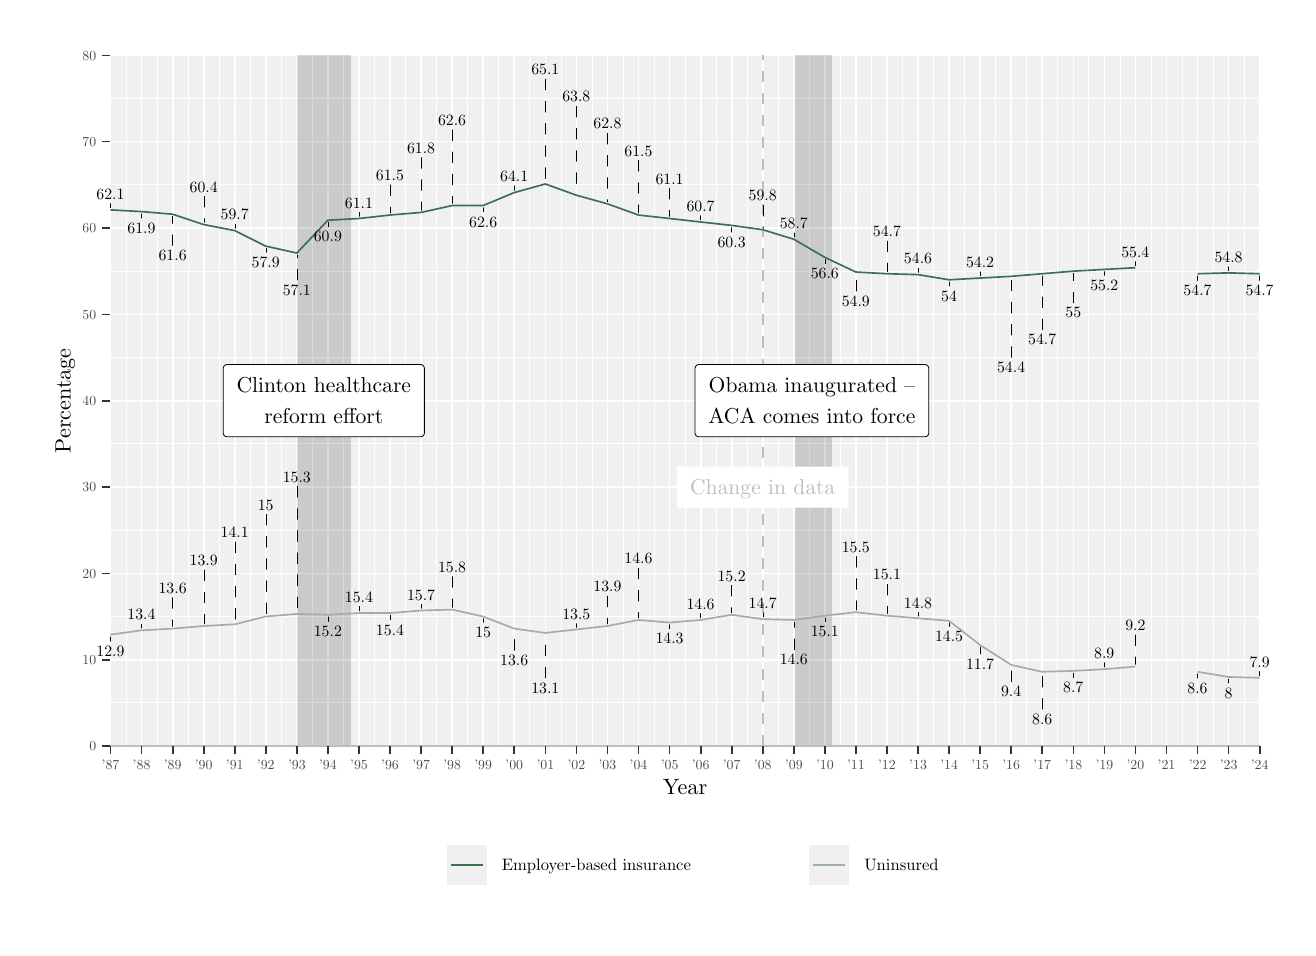
\begin{tikzpicture}[x=1pt,y=1pt]
\definecolor{fillColor}{RGB}{255,255,255}
\path[use as bounding box,fill=fillColor,fill opacity=0.00] (0,0) rectangle (455.30,325.21);
\begin{scope}
\path[clip] (  0.00,  0.00) rectangle (455.30,325.21);
\definecolor{drawColor}{RGB}{255,255,255}
\definecolor{fillColor}{RGB}{255,255,255}

\path[draw=drawColor,line width= 0.6pt,line join=round,line cap=round,fill=fillColor] (  0.00,  0.00) rectangle (455.30,325.21);
\end{scope}
\begin{scope}
\path[clip] (  0.00,  0.00) rectangle (455.30,325.21);
\definecolor{fillColor}{gray}{0.94}

\path[fill=fillColor] ( 29.76, 65.63) rectangle (445.30,315.21);
\definecolor{drawColor}{RGB}{255,255,255}

\path[draw=drawColor,line width= 0.3pt,line join=round] ( 29.76, 81.23) --
	(445.30, 81.23);

\path[draw=drawColor,line width= 0.3pt,line join=round] ( 29.76,112.43) --
	(445.30,112.43);

\path[draw=drawColor,line width= 0.3pt,line join=round] ( 29.76,143.63) --
	(445.30,143.63);

\path[draw=drawColor,line width= 0.3pt,line join=round] ( 29.76,174.83) --
	(445.30,174.83);

\path[draw=drawColor,line width= 0.3pt,line join=round] ( 29.76,206.02) --
	(445.30,206.02);

\path[draw=drawColor,line width= 0.3pt,line join=round] ( 29.76,237.22) --
	(445.30,237.22);

\path[draw=drawColor,line width= 0.3pt,line join=round] ( 29.76,268.42) --
	(445.30,268.42);

\path[draw=drawColor,line width= 0.3pt,line join=round] ( 29.76,299.62) --
	(445.30,299.62);

\path[draw=drawColor,line width= 0.3pt,line join=round] ( 35.56, 65.63) --
	( 35.56,315.21);

\path[draw=drawColor,line width= 0.3pt,line join=round] ( 46.79, 65.63) --
	( 46.79,315.21);

\path[draw=drawColor,line width= 0.3pt,line join=round] ( 58.02, 65.63) --
	( 58.02,315.21);

\path[draw=drawColor,line width= 0.3pt,line join=round] ( 69.23, 65.63) --
	( 69.23,315.21);

\path[draw=drawColor,line width= 0.3pt,line join=round] ( 80.45, 65.63) --
	( 80.45,315.21);

\path[draw=drawColor,line width= 0.3pt,line join=round] ( 91.68, 65.63) --
	( 91.68,315.21);

\path[draw=drawColor,line width= 0.3pt,line join=round] (102.91, 65.63) --
	(102.91,315.21);

\path[draw=drawColor,line width= 0.3pt,line join=round] (114.12, 65.63) --
	(114.12,315.21);

\path[draw=drawColor,line width= 0.3pt,line join=round] (125.34, 65.63) --
	(125.34,315.21);

\path[draw=drawColor,line width= 0.3pt,line join=round] (136.57, 65.63) --
	(136.57,315.21);

\path[draw=drawColor,line width= 0.3pt,line join=round] (147.80, 65.63) --
	(147.80,315.21);

\path[draw=drawColor,line width= 0.3pt,line join=round] (159.01, 65.63) --
	(159.01,315.21);

\path[draw=drawColor,line width= 0.3pt,line join=round] (170.23, 65.63) --
	(170.23,315.21);

\path[draw=drawColor,line width= 0.3pt,line join=round] (181.46, 65.63) --
	(181.46,315.21);

\path[draw=drawColor,line width= 0.3pt,line join=round] (192.69, 65.63) --
	(192.69,315.21);

\path[draw=drawColor,line width= 0.3pt,line join=round] (203.90, 65.63) --
	(203.90,315.21);

\path[draw=drawColor,line width= 0.3pt,line join=round] (215.12, 65.63) --
	(215.12,315.21);

\path[draw=drawColor,line width= 0.3pt,line join=round] (226.35, 65.63) --
	(226.35,315.21);

\path[draw=drawColor,line width= 0.3pt,line join=round] (237.58, 65.63) --
	(237.58,315.21);

\path[draw=drawColor,line width= 0.3pt,line join=round] (248.79, 65.63) --
	(248.79,315.21);

\path[draw=drawColor,line width= 0.3pt,line join=round] (260.01, 65.63) --
	(260.01,315.21);

\path[draw=drawColor,line width= 0.3pt,line join=round] (271.24, 65.63) --
	(271.24,315.21);

\path[draw=drawColor,line width= 0.3pt,line join=round] (282.47, 65.63) --
	(282.47,315.21);

\path[draw=drawColor,line width= 0.3pt,line join=round] (293.68, 65.63) --
	(293.68,315.21);

\path[draw=drawColor,line width= 0.3pt,line join=round] (304.90, 65.63) --
	(304.90,315.21);

\path[draw=drawColor,line width= 0.3pt,line join=round] (316.13, 65.63) --
	(316.13,315.21);

\path[draw=drawColor,line width= 0.3pt,line join=round] (327.36, 65.63) --
	(327.36,315.21);

\path[draw=drawColor,line width= 0.3pt,line join=round] (338.57, 65.63) --
	(338.57,315.21);

\path[draw=drawColor,line width= 0.3pt,line join=round] (349.79, 65.63) --
	(349.79,315.21);

\path[draw=drawColor,line width= 0.3pt,line join=round] (361.02, 65.63) --
	(361.02,315.21);

\path[draw=drawColor,line width= 0.3pt,line join=round] (372.25, 65.63) --
	(372.25,315.21);

\path[draw=drawColor,line width= 0.3pt,line join=round] (383.47, 65.63) --
	(383.47,315.21);

\path[draw=drawColor,line width= 0.3pt,line join=round] (394.68, 65.63) --
	(394.68,315.21);

\path[draw=drawColor,line width= 0.3pt,line join=round] (405.91, 65.63) --
	(405.91,315.21);

\path[draw=drawColor,line width= 0.3pt,line join=round] (417.14, 65.63) --
	(417.14,315.21);

\path[draw=drawColor,line width= 0.3pt,line join=round] (428.36, 65.63) --
	(428.36,315.21);

\path[draw=drawColor,line width= 0.3pt,line join=round] (439.57, 65.63) --
	(439.57,315.21);

\path[draw=drawColor,line width= 0.6pt,line join=round] ( 29.76, 65.63) --
	(445.30, 65.63);

\path[draw=drawColor,line width= 0.6pt,line join=round] ( 29.76, 96.83) --
	(445.30, 96.83);

\path[draw=drawColor,line width= 0.6pt,line join=round] ( 29.76,128.03) --
	(445.30,128.03);

\path[draw=drawColor,line width= 0.6pt,line join=round] ( 29.76,159.23) --
	(445.30,159.23);

\path[draw=drawColor,line width= 0.6pt,line join=round] ( 29.76,190.42) --
	(445.30,190.42);

\path[draw=drawColor,line width= 0.6pt,line join=round] ( 29.76,221.62) --
	(445.30,221.62);

\path[draw=drawColor,line width= 0.6pt,line join=round] ( 29.76,252.82) --
	(445.30,252.82);

\path[draw=drawColor,line width= 0.6pt,line join=round] ( 29.76,284.02) --
	(445.30,284.02);

\path[draw=drawColor,line width= 0.6pt,line join=round] ( 29.76,315.21) --
	(445.30,315.21);

\path[draw=drawColor,line width= 0.6pt,line join=round] ( 29.95, 65.63) --
	( 29.95,315.21);

\path[draw=drawColor,line width= 0.6pt,line join=round] ( 41.16, 65.63) --
	( 41.16,315.21);

\path[draw=drawColor,line width= 0.6pt,line join=round] ( 52.41, 65.63) --
	( 52.41,315.21);

\path[draw=drawColor,line width= 0.6pt,line join=round] ( 63.62, 65.63) --
	( 63.62,315.21);

\path[draw=drawColor,line width= 0.6pt,line join=round] ( 74.84, 65.63) --
	( 74.84,315.21);

\path[draw=drawColor,line width= 0.6pt,line join=round] ( 86.05, 65.63) --
	( 86.05,315.21);

\path[draw=drawColor,line width= 0.6pt,line join=round] ( 97.30, 65.63) --
	( 97.30,315.21);

\path[draw=drawColor,line width= 0.6pt,line join=round] (108.51, 65.63) --
	(108.51,315.21);

\path[draw=drawColor,line width= 0.6pt,line join=round] (119.73, 65.63) --
	(119.73,315.21);

\path[draw=drawColor,line width= 0.6pt,line join=round] (130.94, 65.63) --
	(130.94,315.21);

\path[draw=drawColor,line width= 0.6pt,line join=round] (142.19, 65.63) --
	(142.19,315.21);

\path[draw=drawColor,line width= 0.6pt,line join=round] (153.40, 65.63) --
	(153.40,315.21);

\path[draw=drawColor,line width= 0.6pt,line join=round] (164.62, 65.63) --
	(164.62,315.21);

\path[draw=drawColor,line width= 0.6pt,line join=round] (175.83, 65.63) --
	(175.83,315.21);

\path[draw=drawColor,line width= 0.6pt,line join=round] (187.08, 65.63) --
	(187.08,315.21);

\path[draw=drawColor,line width= 0.6pt,line join=round] (198.30, 65.63) --
	(198.30,315.21);

\path[draw=drawColor,line width= 0.6pt,line join=round] (209.51, 65.63) --
	(209.51,315.21);

\path[draw=drawColor,line width= 0.6pt,line join=round] (220.73, 65.63) --
	(220.73,315.21);

\path[draw=drawColor,line width= 0.6pt,line join=round] (231.97, 65.63) --
	(231.97,315.21);

\path[draw=drawColor,line width= 0.6pt,line join=round] (243.19, 65.63) --
	(243.19,315.21);

\path[draw=drawColor,line width= 0.6pt,line join=round] (254.40, 65.63) --
	(254.40,315.21);

\path[draw=drawColor,line width= 0.6pt,line join=round] (265.62, 65.63) --
	(265.62,315.21);

\path[draw=drawColor,line width= 0.6pt,line join=round] (276.86, 65.63) --
	(276.86,315.21);

\path[draw=drawColor,line width= 0.6pt,line join=round] (288.08, 65.63) --
	(288.08,315.21);

\path[draw=drawColor,line width= 0.6pt,line join=round] (299.29, 65.63) --
	(299.29,315.21);

\path[draw=drawColor,line width= 0.6pt,line join=round] (310.51, 65.63) --
	(310.51,315.21);

\path[draw=drawColor,line width= 0.6pt,line join=round] (321.75, 65.63) --
	(321.75,315.21);

\path[draw=drawColor,line width= 0.6pt,line join=round] (332.97, 65.63) --
	(332.97,315.21);

\path[draw=drawColor,line width= 0.6pt,line join=round] (344.18, 65.63) --
	(344.18,315.21);

\path[draw=drawColor,line width= 0.6pt,line join=round] (355.40, 65.63) --
	(355.40,315.21);

\path[draw=drawColor,line width= 0.6pt,line join=round] (366.64, 65.63) --
	(366.64,315.21);

\path[draw=drawColor,line width= 0.6pt,line join=round] (377.86, 65.63) --
	(377.86,315.21);

\path[draw=drawColor,line width= 0.6pt,line join=round] (389.07, 65.63) --
	(389.07,315.21);

\path[draw=drawColor,line width= 0.6pt,line join=round] (400.29, 65.63) --
	(400.29,315.21);

\path[draw=drawColor,line width= 0.6pt,line join=round] (411.53, 65.63) --
	(411.53,315.21);

\path[draw=drawColor,line width= 0.6pt,line join=round] (422.75, 65.63) --
	(422.75,315.21);

\path[draw=drawColor,line width= 0.6pt,line join=round] (433.96, 65.63) --
	(433.96,315.21);

\path[draw=drawColor,line width= 0.6pt,line join=round] (445.18, 65.63) --
	(445.18,315.21);
\definecolor{fillColor}{RGB}{190,190,190}

\path[fill=fillColor,fill opacity=0.01] ( 97.30, 65.63) rectangle (116.75,315.21);

\path[fill=fillColor,fill opacity=0.01] ( 97.30, 65.63) rectangle (116.75,315.21);

\path[fill=fillColor,fill opacity=0.01] ( 97.30, 65.63) rectangle (116.75,315.21);

\path[fill=fillColor,fill opacity=0.01] ( 97.30, 65.63) rectangle (116.75,315.21);

\path[fill=fillColor,fill opacity=0.01] ( 97.30, 65.63) rectangle (116.75,315.21);

\path[fill=fillColor,fill opacity=0.01] ( 97.30, 65.63) rectangle (116.75,315.21);

\path[fill=fillColor,fill opacity=0.01] ( 97.30, 65.63) rectangle (116.75,315.21);

\path[fill=fillColor,fill opacity=0.01] ( 97.30, 65.63) rectangle (116.75,315.21);

\path[fill=fillColor,fill opacity=0.01] ( 97.30, 65.63) rectangle (116.75,315.21);

\path[fill=fillColor,fill opacity=0.01] ( 97.30, 65.63) rectangle (116.75,315.21);

\path[fill=fillColor,fill opacity=0.01] ( 97.30, 65.63) rectangle (116.75,315.21);

\path[fill=fillColor,fill opacity=0.01] ( 97.30, 65.63) rectangle (116.75,315.21);

\path[fill=fillColor,fill opacity=0.01] ( 97.30, 65.63) rectangle (116.75,315.21);

\path[fill=fillColor,fill opacity=0.01] ( 97.30, 65.63) rectangle (116.75,315.21);

\path[fill=fillColor,fill opacity=0.01] ( 97.30, 65.63) rectangle (116.75,315.21);

\path[fill=fillColor,fill opacity=0.01] ( 97.30, 65.63) rectangle (116.75,315.21);

\path[fill=fillColor,fill opacity=0.01] ( 97.30, 65.63) rectangle (116.75,315.21);

\path[fill=fillColor,fill opacity=0.01] ( 97.30, 65.63) rectangle (116.75,315.21);

\path[fill=fillColor,fill opacity=0.01] ( 97.30, 65.63) rectangle (116.75,315.21);

\path[fill=fillColor,fill opacity=0.01] ( 97.30, 65.63) rectangle (116.75,315.21);

\path[fill=fillColor,fill opacity=0.01] ( 97.30, 65.63) rectangle (116.75,315.21);

\path[fill=fillColor,fill opacity=0.01] ( 97.30, 65.63) rectangle (116.75,315.21);

\path[fill=fillColor,fill opacity=0.01] ( 97.30, 65.63) rectangle (116.75,315.21);

\path[fill=fillColor,fill opacity=0.01] ( 97.30, 65.63) rectangle (116.75,315.21);

\path[fill=fillColor,fill opacity=0.01] ( 97.30, 65.63) rectangle (116.75,315.21);

\path[fill=fillColor,fill opacity=0.01] ( 97.30, 65.63) rectangle (116.75,315.21);

\path[fill=fillColor,fill opacity=0.01] ( 97.30, 65.63) rectangle (116.75,315.21);

\path[fill=fillColor,fill opacity=0.01] ( 97.30, 65.63) rectangle (116.75,315.21);

\path[fill=fillColor,fill opacity=0.01] ( 97.30, 65.63) rectangle (116.75,315.21);

\path[fill=fillColor,fill opacity=0.01] ( 97.30, 65.63) rectangle (116.75,315.21);

\path[fill=fillColor,fill opacity=0.01] ( 97.30, 65.63) rectangle (116.75,315.21);

\path[fill=fillColor,fill opacity=0.01] ( 97.30, 65.63) rectangle (116.75,315.21);

\path[fill=fillColor,fill opacity=0.01] ( 97.30, 65.63) rectangle (116.75,315.21);

\path[fill=fillColor,fill opacity=0.01] ( 97.30, 65.63) rectangle (116.75,315.21);

\path[fill=fillColor,fill opacity=0.01] ( 97.30, 65.63) rectangle (116.75,315.21);

\path[fill=fillColor,fill opacity=0.01] ( 97.30, 65.63) rectangle (116.75,315.21);

\path[fill=fillColor,fill opacity=0.01] ( 97.30, 65.63) rectangle (116.75,315.21);

\path[fill=fillColor,fill opacity=0.01] ( 97.30, 65.63) rectangle (116.75,315.21);

\path[fill=fillColor,fill opacity=0.01] (277.45, 65.63) rectangle (290.57,315.21);

\path[fill=fillColor,fill opacity=0.01] (277.45, 65.63) rectangle (290.57,315.21);

\path[fill=fillColor,fill opacity=0.01] (277.45, 65.63) rectangle (290.57,315.21);

\path[fill=fillColor,fill opacity=0.01] (277.45, 65.63) rectangle (290.57,315.21);

\path[fill=fillColor,fill opacity=0.01] (277.45, 65.63) rectangle (290.57,315.21);

\path[fill=fillColor,fill opacity=0.01] (277.45, 65.63) rectangle (290.57,315.21);

\path[fill=fillColor,fill opacity=0.01] (277.45, 65.63) rectangle (290.57,315.21);

\path[fill=fillColor,fill opacity=0.01] (277.45, 65.63) rectangle (290.57,315.21);

\path[fill=fillColor,fill opacity=0.01] (277.45, 65.63) rectangle (290.57,315.21);

\path[fill=fillColor,fill opacity=0.01] (277.45, 65.63) rectangle (290.57,315.21);

\path[fill=fillColor,fill opacity=0.01] (277.45, 65.63) rectangle (290.57,315.21);

\path[fill=fillColor,fill opacity=0.01] (277.45, 65.63) rectangle (290.57,315.21);

\path[fill=fillColor,fill opacity=0.01] (277.45, 65.63) rectangle (290.57,315.21);

\path[fill=fillColor,fill opacity=0.01] (277.45, 65.63) rectangle (290.57,315.21);

\path[fill=fillColor,fill opacity=0.01] (277.45, 65.63) rectangle (290.57,315.21);

\path[fill=fillColor,fill opacity=0.01] (277.45, 65.63) rectangle (290.57,315.21);

\path[fill=fillColor,fill opacity=0.01] (277.45, 65.63) rectangle (290.57,315.21);

\path[fill=fillColor,fill opacity=0.01] (277.45, 65.63) rectangle (290.57,315.21);

\path[fill=fillColor,fill opacity=0.01] (277.45, 65.63) rectangle (290.57,315.21);

\path[fill=fillColor,fill opacity=0.01] (277.45, 65.63) rectangle (290.57,315.21);

\path[fill=fillColor,fill opacity=0.01] (277.45, 65.63) rectangle (290.57,315.21);

\path[fill=fillColor,fill opacity=0.01] (277.45, 65.63) rectangle (290.57,315.21);

\path[fill=fillColor,fill opacity=0.01] (277.45, 65.63) rectangle (290.57,315.21);

\path[fill=fillColor,fill opacity=0.01] (277.45, 65.63) rectangle (290.57,315.21);

\path[fill=fillColor,fill opacity=0.01] (277.45, 65.63) rectangle (290.57,315.21);

\path[fill=fillColor,fill opacity=0.01] (277.45, 65.63) rectangle (290.57,315.21);

\path[fill=fillColor,fill opacity=0.01] (277.45, 65.63) rectangle (290.57,315.21);

\path[fill=fillColor,fill opacity=0.01] (277.45, 65.63) rectangle (290.57,315.21);

\path[fill=fillColor,fill opacity=0.01] (277.45, 65.63) rectangle (290.57,315.21);

\path[fill=fillColor,fill opacity=0.01] (277.45, 65.63) rectangle (290.57,315.21);

\path[fill=fillColor,fill opacity=0.01] (277.45, 65.63) rectangle (290.57,315.21);

\path[fill=fillColor,fill opacity=0.01] (277.45, 65.63) rectangle (290.57,315.21);

\path[fill=fillColor,fill opacity=0.01] (277.45, 65.63) rectangle (290.57,315.21);

\path[fill=fillColor,fill opacity=0.01] (277.45, 65.63) rectangle (290.57,315.21);

\path[fill=fillColor,fill opacity=0.01] (277.45, 65.63) rectangle (290.57,315.21);

\path[fill=fillColor,fill opacity=0.01] (277.45, 65.63) rectangle (290.57,315.21);

\path[fill=fillColor,fill opacity=0.01] (277.45, 65.63) rectangle (290.57,315.21);

\path[fill=fillColor,fill opacity=0.01] (277.45, 65.63) rectangle (290.57,315.21);
\definecolor{drawColor}{RGB}{190,190,190}

\path[draw=drawColor,line width= 0.6pt,dash pattern=on 4pt off 4pt ,line join=round] (265.59, 65.63) -- (265.59,315.21);

\path[draw=drawColor,line width= 0.6pt,line join=round] ( 29.76, 65.63) -- (445.30, 65.63);
\definecolor{drawColor}{RGB}{60,113,79}

\path[draw=drawColor,line width= 0.6pt,line join=round] ( 29.92,259.37) --
	( 41.13,258.75) --
	( 52.38,257.81) --
	( 63.59,254.07) --
	( 74.81,251.88) --
	( 86.02,246.27) --
	( 97.27,243.77) --
	(108.48,255.63) --
	(119.70,256.25) --
	(130.91,257.50) --
	(142.16,258.44) --
	(153.37,260.93) --
	(164.59,260.93) --
	(175.80,265.61) --
	(187.05,268.73) --
	(198.26,264.67) --
	(209.48,261.56) --
	(220.69,257.50) --
	(231.94,256.25) --
	(243.16,255.00) --
	(254.37,253.76) --
	(265.59,252.20) --
	(276.83,248.76) --
	(288.05,242.21) --
	(299.26,236.91) --
	(310.48,236.29) --
	(321.72,235.97) --
	(332.94,234.10) --
	(344.15,234.73) --
	(355.37,235.35) --
	(366.61,236.29) --
	(377.83,237.22) --
	(389.04,237.85) --
	(400.26,238.47);

\path[draw=drawColor,line width= 0.6pt,line join=round] (422.72,236.29) --
	(433.93,236.60) --
	(445.15,236.29);
\definecolor{drawColor}{RGB}{157,176,162}

\path[draw=drawColor,line width= 0.6pt,line join=round] ( 29.92,105.88) --
	( 41.13,107.44) --
	( 52.38,108.06) --
	( 63.59,109.00) --
	( 74.81,109.62) --
	( 86.02,112.43) --
	( 97.27,113.37) --
	(108.48,113.05) --
	(119.70,113.68) --
	(130.91,113.68) --
	(142.16,114.61) --
	(153.37,114.93) --
	(164.59,112.43) --
	(175.80,108.06) --
	(187.05,106.50) --
	(198.26,107.75) --
	(209.48,109.00) --
	(220.69,111.18) --
	(231.94,110.25) --
	(243.16,111.18) --
	(254.37,113.05) --
	(265.59,111.49) --
	(276.83,111.18) --
	(288.05,112.74) --
	(299.26,113.99) --
	(310.48,112.74) --
	(321.72,111.81) --
	(332.94,110.87) --
	(344.15,102.14) --
	(355.37, 94.96) --
	(366.61, 92.46) --
	(377.83, 92.78) --
	(389.04, 93.40) --
	(400.26, 94.34);

\path[draw=drawColor,line width= 0.6pt,line join=round] (422.72, 92.46) --
	(433.93, 90.59) --
	(445.15, 90.28);
\definecolor{drawColor}{RGB}{0,0,0}

\path[draw=drawColor,line width= 0.1pt,dash pattern=on 4pt off 4pt ,line join=round,line cap=round] ( 29.92,103.45) -- ( 29.92,105.15);

\path[draw=drawColor,line width= 0.1pt,dash pattern=on 4pt off 4pt ,line join=round,line cap=round] ( 41.13,109.69) -- ( 41.13,108.17);

\path[draw=drawColor,line width= 0.1pt,dash pattern=on 4pt off 4pt ,line join=round,line cap=round] ( 52.38,119.31) -- ( 52.38,108.79);

\path[draw=drawColor,line width= 0.1pt,dash pattern=on 4pt off 4pt ,line join=round,line cap=round] ( 63.59,129.31) -- ( 63.59,109.73);

\path[draw=drawColor,line width= 0.1pt,dash pattern=on 4pt off 4pt ,line join=round,line cap=round] ( 74.81,139.40) -- ( 74.81,110.35);

\path[draw=drawColor,line width= 0.1pt,dash pattern=on 4pt off 4pt ,line join=round,line cap=round] ( 86.02,149.41) -- ( 86.02,113.16);

\path[draw=drawColor,line width= 0.1pt,dash pattern=on 4pt off 4pt ,line join=round,line cap=round] ( 97.27,159.50) -- ( 97.27,114.09);

\path[draw=drawColor,line width= 0.1pt,dash pattern=on 4pt off 4pt ,line join=round,line cap=round] (108.48,110.54) -- (108.48,112.33);

\path[draw=drawColor,line width= 0.1pt,dash pattern=on 4pt off 4pt ,line join=round,line cap=round] (119.70,116.14) -- (119.70,114.41);

\path[draw=drawColor,line width= 0.1pt,dash pattern=on 4pt off 4pt ,line join=round,line cap=round] (130.91,111.17) -- (130.91,112.95);

\path[draw=drawColor,line width= 0.1pt,dash pattern=on 4pt off 4pt ,line join=round,line cap=round] (142.16,116.84) -- (142.16,115.34);

\path[draw=drawColor,line width= 0.1pt,dash pattern=on 4pt off 4pt ,line join=round,line cap=round] (153.37,126.89) -- (153.37,115.65);

\path[draw=drawColor,line width= 0.1pt,dash pattern=on 4pt off 4pt ,line join=round,line cap=round] (164.59,110.27) -- (164.59,111.70);

\path[draw=drawColor,line width= 0.1pt,dash pattern=on 4pt off 4pt ,line join=round,line cap=round] (175.80,100.17) -- (175.80,107.34);

\path[draw=drawColor,line width= 0.1pt,dash pattern=on 4pt off 4pt ,line join=round,line cap=round] (187.05, 90.19) -- (187.05,105.78);

\path[draw=drawColor,line width= 0.1pt,dash pattern=on 4pt off 4pt ,line join=round,line cap=round] (198.26,109.94) -- (198.26,108.48);

\path[draw=drawColor,line width= 0.1pt,dash pattern=on 4pt off 4pt ,line join=round,line cap=round] (209.48,119.89) -- (209.48,109.73);

\path[draw=drawColor,line width= 0.1pt,dash pattern=on 4pt off 4pt ,line join=round,line cap=round] (220.69,129.93) -- (220.69,111.91);

\path[draw=drawColor,line width= 0.1pt,dash pattern=on 4pt off 4pt ,line join=round,line cap=round] (231.94,108.00) -- (231.94,109.52);

\path[draw=drawColor,line width= 0.1pt,dash pattern=on 4pt off 4pt ,line join=round,line cap=round] (243.16,113.58) -- (243.16,111.91);

\path[draw=drawColor,line width= 0.1pt,dash pattern=on 4pt off 4pt ,line join=round,line cap=round] (254.37,123.72) -- (254.37,113.78);

\path[draw=drawColor,line width= 0.1pt,dash pattern=on 4pt off 4pt ,line join=round,line cap=round] (265.59,113.85) -- (265.59,112.22);

\path[draw=drawColor,line width= 0.1pt,dash pattern=on 4pt off 4pt ,line join=round,line cap=round] (276.83,100.42) -- (276.83,110.46);

\path[draw=drawColor,line width= 0.1pt,dash pattern=on 4pt off 4pt ,line join=round,line cap=round] (288.05,110.56) -- (288.05,112.02);

\path[draw=drawColor,line width= 0.1pt,dash pattern=on 4pt off 4pt ,line join=round,line cap=round] (299.26,134.18) -- (299.26,114.72);

\path[draw=drawColor,line width= 0.1pt,dash pattern=on 4pt off 4pt ,line join=round,line cap=round] (310.48,124.12) -- (310.48,113.47);

\path[draw=drawColor,line width= 0.1pt,dash pattern=on 4pt off 4pt ,line join=round,line cap=round] (321.72,113.98) -- (321.72,112.53);

\path[draw=drawColor,line width= 0.1pt,dash pattern=on 4pt off 4pt ,line join=round,line cap=round] (332.94,108.76) -- (332.94,110.14);

\path[draw=drawColor,line width= 0.1pt,dash pattern=on 4pt off 4pt ,line join=round,line cap=round] (344.15, 98.85) -- (344.15,101.41);

\path[draw=drawColor,line width= 0.1pt,dash pattern=on 4pt off 4pt ,line join=round,line cap=round] (355.37, 88.86) -- (355.37, 94.23);

\path[draw=drawColor,line width= 0.1pt,dash pattern=on 4pt off 4pt ,line join=round,line cap=round] (366.61, 78.87) -- (366.61, 91.74);

\path[draw=drawColor,line width= 0.1pt,dash pattern=on 4pt off 4pt ,line join=round,line cap=round] (377.83, 90.27) -- (377.83, 92.05);

\path[draw=drawColor,line width= 0.1pt,dash pattern=on 4pt off 4pt ,line join=round,line cap=round] (389.04, 95.83) -- (389.04, 94.13);

\path[draw=drawColor,line width= 0.1pt,dash pattern=on 4pt off 4pt ,line join=round,line cap=round] (400.26,105.86) -- (400.26, 95.06);

\path[draw=drawColor,line width= 0.1pt,dash pattern=on 4pt off 4pt ,line join=round,line cap=round] (422.72, 90.14) -- (422.72, 91.74);

\path[draw=drawColor,line width= 0.1pt,dash pattern=on 4pt off 4pt ,line join=round,line cap=round] (433.93, 88.36) -- (433.93, 89.87);

\path[draw=drawColor,line width= 0.1pt,dash pattern=on 4pt off 4pt ,line join=round,line cap=round] (445.15, 92.61) -- (445.15, 91.01);

\node[text=drawColor,anchor=base,inner sep=0pt, outer sep=0pt, scale=  0.57] at ( 29.92, 98.03) {12.9};

\node[text=drawColor,anchor=base,inner sep=0pt, outer sep=0pt, scale=  0.57] at ( 41.13,111.19) {13.4};

\node[text=drawColor,anchor=base,inner sep=0pt, outer sep=0pt, scale=  0.57] at ( 52.38,120.82) {13.6};

\node[text=drawColor,anchor=base,inner sep=0pt, outer sep=0pt, scale=  0.57] at ( 63.59,130.82) {13.9};

\node[text=drawColor,anchor=base,inner sep=0pt, outer sep=0pt, scale=  0.57] at ( 74.81,140.91) {14.1};

\node[text=drawColor,anchor=base,inner sep=0pt, outer sep=0pt, scale=  0.57] at ( 86.02,150.92) {15};

\node[text=drawColor,anchor=base,inner sep=0pt, outer sep=0pt, scale=  0.57] at ( 97.27,161.01) {15.3};

\node[text=drawColor,anchor=base,inner sep=0pt, outer sep=0pt, scale=  0.57] at (108.48,105.12) {15.2};

\node[text=drawColor,anchor=base,inner sep=0pt, outer sep=0pt, scale=  0.57] at (119.70,117.65) {15.4};

\node[text=drawColor,anchor=base,inner sep=0pt, outer sep=0pt, scale=  0.57] at (130.91,105.74) {15.4};

\node[text=drawColor,anchor=base,inner sep=0pt, outer sep=0pt, scale=  0.57] at (142.16,118.34) {15.7};

\node[text=drawColor,anchor=base,inner sep=0pt, outer sep=0pt, scale=  0.57] at (153.37,128.39) {15.8};

\node[text=drawColor,anchor=base,inner sep=0pt, outer sep=0pt, scale=  0.57] at (164.59,104.84) {15};

\node[text=drawColor,anchor=base,inner sep=0pt, outer sep=0pt, scale=  0.57] at (175.80, 94.75) {13.6};

\node[text=drawColor,anchor=base,inner sep=0pt, outer sep=0pt, scale=  0.57] at (187.05, 84.76) {13.1};

\node[text=drawColor,anchor=base,inner sep=0pt, outer sep=0pt, scale=  0.57] at (198.26,111.44) {13.5};

\node[text=drawColor,anchor=base,inner sep=0pt, outer sep=0pt, scale=  0.57] at (209.48,121.39) {13.9};

\node[text=drawColor,anchor=base,inner sep=0pt, outer sep=0pt, scale=  0.57] at (220.69,131.44) {14.6};

\node[text=drawColor,anchor=base,inner sep=0pt, outer sep=0pt, scale=  0.57] at (231.94,102.57) {14.3};

\node[text=drawColor,anchor=base,inner sep=0pt, outer sep=0pt, scale=  0.57] at (243.16,115.08) {14.6};

\node[text=drawColor,anchor=base,inner sep=0pt, outer sep=0pt, scale=  0.57] at (254.37,125.22) {15.2};

\node[text=drawColor,anchor=base,inner sep=0pt, outer sep=0pt, scale=  0.57] at (265.59,115.36) {14.7};

\node[text=drawColor,anchor=base,inner sep=0pt, outer sep=0pt, scale=  0.57] at (276.83, 95.00) {14.6};

\node[text=drawColor,anchor=base,inner sep=0pt, outer sep=0pt, scale=  0.57] at (288.05,105.14) {15.1};

\node[text=drawColor,anchor=base,inner sep=0pt, outer sep=0pt, scale=  0.57] at (299.26,135.69) {15.5};

\node[text=drawColor,anchor=base,inner sep=0pt, outer sep=0pt, scale=  0.57] at (310.48,125.63) {15.1};

\node[text=drawColor,anchor=base,inner sep=0pt, outer sep=0pt, scale=  0.57] at (321.72,115.48) {14.8};

\node[text=drawColor,anchor=base,inner sep=0pt, outer sep=0pt, scale=  0.57] at (332.94,103.33) {14.5};

\node[text=drawColor,anchor=base,inner sep=0pt, outer sep=0pt, scale=  0.57] at (344.15, 93.43) {11.7};

\node[text=drawColor,anchor=base,inner sep=0pt, outer sep=0pt, scale=  0.57] at (355.37, 83.43) {9.4};

\node[text=drawColor,anchor=base,inner sep=0pt, outer sep=0pt, scale=  0.57] at (366.61, 73.45) {8.6};

\node[text=drawColor,anchor=base,inner sep=0pt, outer sep=0pt, scale=  0.57] at (377.83, 84.85) {8.7};

\node[text=drawColor,anchor=base,inner sep=0pt, outer sep=0pt, scale=  0.57] at (389.04, 97.34) {8.9};

\node[text=drawColor,anchor=base,inner sep=0pt, outer sep=0pt, scale=  0.57] at (400.26,107.37) {9.2};

\node[text=drawColor,anchor=base,inner sep=0pt, outer sep=0pt, scale=  0.57] at (422.72, 84.71) {8.6};

\node[text=drawColor,anchor=base,inner sep=0pt, outer sep=0pt, scale=  0.57] at (433.93, 82.93) {8};

\node[text=drawColor,anchor=base,inner sep=0pt, outer sep=0pt, scale=  0.57] at (445.15, 94.11) {7.9};

\path[draw=drawColor,line width= 0.1pt,dash pattern=on 4pt off 4pt ,line join=round,line cap=round] ( 29.92,261.65) -- ( 29.92,260.10);

\path[draw=drawColor,line width= 0.1pt,dash pattern=on 4pt off 4pt ,line join=round,line cap=round] ( 41.13,256.34) -- ( 41.13,258.02);

\path[draw=drawColor,line width= 0.1pt,dash pattern=on 4pt off 4pt ,line join=round,line cap=round] ( 52.38,246.44) -- ( 52.38,257.09);

\path[draw=drawColor,line width= 0.1pt,dash pattern=on 4pt off 4pt ,line join=round,line cap=round] ( 63.59,264.30) -- ( 63.59,254.79);

\path[draw=drawColor,line width= 0.1pt,dash pattern=on 4pt off 4pt ,line join=round,line cap=round] ( 74.81,254.28) -- ( 74.81,252.61);

\path[draw=drawColor,line width= 0.1pt,dash pattern=on 4pt off 4pt ,line join=round,line cap=round] ( 86.02,243.94) -- ( 86.02,245.54);

\path[draw=drawColor,line width= 0.1pt,dash pattern=on 4pt off 4pt ,line join=round,line cap=round] ( 97.27,234.01) -- ( 97.27,243.05);

\path[draw=drawColor,line width= 0.1pt,dash pattern=on 4pt off 4pt ,line join=round,line cap=round] (108.48,253.22) -- (108.48,254.90);

\path[draw=drawColor,line width= 0.1pt,dash pattern=on 4pt off 4pt ,line join=round,line cap=round] (119.70,258.51) -- (119.70,256.98);

\path[draw=drawColor,line width= 0.1pt,dash pattern=on 4pt off 4pt ,line join=round,line cap=round] (130.91,268.43) -- (130.91,258.23);

\path[draw=drawColor,line width= 0.1pt,dash pattern=on 4pt off 4pt ,line join=round,line cap=round] (142.16,278.34) -- (142.16,259.16);

\path[draw=drawColor,line width= 0.1pt,dash pattern=on 4pt off 4pt ,line join=round,line cap=round] (153.37,288.33) -- (153.37,261.66);

\path[draw=drawColor,line width= 0.1pt,dash pattern=on 4pt off 4pt ,line join=round,line cap=round] (164.59,258.61) -- (164.59,260.20);

\path[draw=drawColor,line width= 0.1pt,dash pattern=on 4pt off 4pt ,line join=round,line cap=round] (175.80,268.11) -- (175.80,266.34);

\path[draw=drawColor,line width= 0.1pt,dash pattern=on 4pt off 4pt ,line join=round,line cap=round] (187.05,306.66) -- (187.05,269.46);

\path[draw=drawColor,line width= 0.1pt,dash pattern=on 4pt off 4pt ,line join=round,line cap=round] (198.26,296.85) -- (198.26,265.40);

\path[draw=drawColor,line width= 0.1pt,dash pattern=on 4pt off 4pt ,line join=round,line cap=round] (209.48,287.10) -- (209.48,262.28);

\path[draw=drawColor,line width= 0.1pt,dash pattern=on 4pt off 4pt ,line join=round,line cap=round] (220.69,277.28) -- (220.69,258.23);

\path[draw=drawColor,line width= 0.1pt,dash pattern=on 4pt off 4pt ,line join=round,line cap=round] (231.94,267.21) -- (231.94,256.98);

\path[draw=drawColor,line width= 0.1pt,dash pattern=on 4pt off 4pt ,line join=round,line cap=round] (243.16,257.33) -- (243.16,255.73);

\path[draw=drawColor,line width= 0.1pt,dash pattern=on 4pt off 4pt ,line join=round,line cap=round] (254.37,251.28) -- (254.37,253.03);

\path[draw=drawColor,line width= 0.1pt,dash pattern=on 4pt off 4pt ,line join=round,line cap=round] (265.59,261.07) -- (265.59,252.92);

\path[draw=drawColor,line width= 0.1pt,dash pattern=on 4pt off 4pt ,line join=round,line cap=round] (276.83,251.07) -- (276.83,249.49);

\path[draw=drawColor,line width= 0.1pt,dash pattern=on 4pt off 4pt ,line join=round,line cap=round] (288.05,239.91) -- (288.05,241.49);

\path[draw=drawColor,line width= 0.1pt,dash pattern=on 4pt off 4pt ,line join=round,line cap=round] (299.26,229.94) -- (299.26,236.18);

\path[draw=drawColor,line width= 0.1pt,dash pattern=on 4pt off 4pt ,line join=round,line cap=round] (310.48,248.16) -- (310.48,237.01);

\path[draw=drawColor,line width= 0.1pt,dash pattern=on 4pt off 4pt ,line join=round,line cap=round] (321.72,238.33) -- (321.72,236.70);

\path[draw=drawColor,line width= 0.1pt,dash pattern=on 4pt off 4pt ,line join=round,line cap=round] (332.94,231.78) -- (332.94,233.38);

\path[draw=drawColor,line width= 0.1pt,dash pattern=on 4pt off 4pt ,line join=round,line cap=round] (344.15,237.05) -- (344.15,235.45);

\path[draw=drawColor,line width= 0.1pt,dash pattern=on 4pt off 4pt ,line join=round,line cap=round] (355.37,206.03) -- (355.37,234.62);

\path[draw=drawColor,line width= 0.1pt,dash pattern=on 4pt off 4pt ,line join=round,line cap=round] (366.61,215.98) -- (366.61,235.56);

\path[draw=drawColor,line width= 0.1pt,dash pattern=on 4pt off 4pt ,line join=round,line cap=round] (377.83,225.72) -- (377.83,236.49);

\path[draw=drawColor,line width= 0.1pt,dash pattern=on 4pt off 4pt ,line join=round,line cap=round] (389.04,235.65) -- (389.04,237.12);

\path[draw=drawColor,line width= 0.1pt,dash pattern=on 4pt off 4pt ,line join=round,line cap=round] (400.26,240.75) -- (400.26,239.20);

\path[draw=drawColor,line width= 0.1pt,dash pattern=on 4pt off 4pt ,line join=round,line cap=round] (422.72,233.80) -- (422.72,235.56);

\path[draw=drawColor,line width= 0.1pt,dash pattern=on 4pt off 4pt ,line join=round,line cap=round] (433.93,238.88) -- (433.93,237.32);

\path[draw=drawColor,line width= 0.1pt,dash pattern=on 4pt off 4pt ,line join=round,line cap=round] (445.15,233.85) -- (445.15,235.56);

\node[text=drawColor,anchor=base,inner sep=0pt, outer sep=0pt, scale=  0.57] at ( 29.92,263.16) {62.1};

\node[text=drawColor,anchor=base,inner sep=0pt, outer sep=0pt, scale=  0.57] at ( 41.13,250.92) {61.9};

\node[text=drawColor,anchor=base,inner sep=0pt, outer sep=0pt, scale=  0.57] at ( 52.38,241.02) {61.6};

\node[text=drawColor,anchor=base,inner sep=0pt, outer sep=0pt, scale=  0.57] at ( 63.59,265.80) {60.4};

\node[text=drawColor,anchor=base,inner sep=0pt, outer sep=0pt, scale=  0.57] at ( 74.81,255.78) {59.7};

\node[text=drawColor,anchor=base,inner sep=0pt, outer sep=0pt, scale=  0.57] at ( 86.02,238.51) {57.9};

\node[text=drawColor,anchor=base,inner sep=0pt, outer sep=0pt, scale=  0.57] at ( 97.27,228.58) {57.1};

\node[text=drawColor,anchor=base,inner sep=0pt, outer sep=0pt, scale=  0.57] at (108.48,247.80) {60.9};

\node[text=drawColor,anchor=base,inner sep=0pt, outer sep=0pt, scale=  0.57] at (119.70,260.01) {61.1};

\node[text=drawColor,anchor=base,inner sep=0pt, outer sep=0pt, scale=  0.57] at (130.91,269.93) {61.5};

\node[text=drawColor,anchor=base,inner sep=0pt, outer sep=0pt, scale=  0.57] at (142.16,279.84) {61.8};

\node[text=drawColor,anchor=base,inner sep=0pt, outer sep=0pt, scale=  0.57] at (153.37,289.84) {62.6};

\node[text=drawColor,anchor=base,inner sep=0pt, outer sep=0pt, scale=  0.57] at (164.59,253.18) {62.6};

\node[text=drawColor,anchor=base,inner sep=0pt, outer sep=0pt, scale=  0.57] at (175.80,269.62) {64.1};

\node[text=drawColor,anchor=base,inner sep=0pt, outer sep=0pt, scale=  0.57] at (187.05,308.17) {65.1};

\node[text=drawColor,anchor=base,inner sep=0pt, outer sep=0pt, scale=  0.57] at (198.26,298.36) {63.8};

\node[text=drawColor,anchor=base,inner sep=0pt, outer sep=0pt, scale=  0.57] at (209.48,288.61) {62.8};

\node[text=drawColor,anchor=base,inner sep=0pt, outer sep=0pt, scale=  0.57] at (220.69,278.78) {61.5};

\node[text=drawColor,anchor=base,inner sep=0pt, outer sep=0pt, scale=  0.57] at (231.94,268.71) {61.1};

\node[text=drawColor,anchor=base,inner sep=0pt, outer sep=0pt, scale=  0.57] at (243.16,258.84) {60.7};

\node[text=drawColor,anchor=base,inner sep=0pt, outer sep=0pt, scale=  0.57] at (254.37,245.85) {60.3};

\node[text=drawColor,anchor=base,inner sep=0pt, outer sep=0pt, scale=  0.57] at (265.59,262.58) {59.8};

\node[text=drawColor,anchor=base,inner sep=0pt, outer sep=0pt, scale=  0.57] at (276.83,252.58) {58.7};

\node[text=drawColor,anchor=base,inner sep=0pt, outer sep=0pt, scale=  0.57] at (288.05,234.49) {56.6};

\node[text=drawColor,anchor=base,inner sep=0pt, outer sep=0pt, scale=  0.57] at (299.26,224.51) {54.9};

\node[text=drawColor,anchor=base,inner sep=0pt, outer sep=0pt, scale=  0.57] at (310.48,249.66) {54.7};

\node[text=drawColor,anchor=base,inner sep=0pt, outer sep=0pt, scale=  0.57] at (321.72,239.83) {54.6};

\node[text=drawColor,anchor=base,inner sep=0pt, outer sep=0pt, scale=  0.57] at (332.94,226.36) {54};

\node[text=drawColor,anchor=base,inner sep=0pt, outer sep=0pt, scale=  0.57] at (344.15,238.56) {54.2};

\node[text=drawColor,anchor=base,inner sep=0pt, outer sep=0pt, scale=  0.57] at (355.37,200.60) {54.4};

\node[text=drawColor,anchor=base,inner sep=0pt, outer sep=0pt, scale=  0.57] at (366.61,210.56) {54.7};

\node[text=drawColor,anchor=base,inner sep=0pt, outer sep=0pt, scale=  0.57] at (377.83,220.30) {55};

\node[text=drawColor,anchor=base,inner sep=0pt, outer sep=0pt, scale=  0.57] at (389.04,230.23) {55.2};

\node[text=drawColor,anchor=base,inner sep=0pt, outer sep=0pt, scale=  0.57] at (400.26,242.26) {55.4};

\node[text=drawColor,anchor=base,inner sep=0pt, outer sep=0pt, scale=  0.57] at (422.72,228.37) {54.7};

\node[text=drawColor,anchor=base,inner sep=0pt, outer sep=0pt, scale=  0.57] at (433.93,240.39) {54.8};

\node[text=drawColor,anchor=base,inner sep=0pt, outer sep=0pt, scale=  0.57] at (445.15,228.43) {54.7};
\definecolor{fillColor}{RGB}{255,255,255}

\path[fill=fillColor] (234.58,151.82) --
	(296.59,151.82) --
	(296.59,151.82) --
	(296.59,151.82) --
	(296.59,151.82) --
	(296.59,151.82) --
	(296.59,151.82) --
	(296.59,151.82) --
	(296.59,151.82) --
	(296.59,151.82) --
	(296.59,151.82) --
	(296.59,151.82) --
	(296.59,151.82) --
	(296.59,151.82) --
	(296.59,166.63) --
	(296.59,166.63) --
	(296.59,166.63) --
	(296.59,166.63) --
	(296.59,166.63) --
	(296.59,166.63) --
	(296.59,166.63) --
	(296.59,166.63) --
	(296.59,166.63) --
	(296.59,166.63) --
	(296.59,166.63) --
	(296.59,166.63) --
	(234.58,166.63) --
	(234.58,166.63) --
	(234.58,166.63) --
	(234.58,166.63) --
	(234.58,166.63) --
	(234.58,166.63) --
	(234.58,166.63) --
	(234.58,166.63) --
	(234.58,166.63) --
	(234.58,166.63) --
	(234.58,166.63) --
	(234.58,166.63) --
	(234.58,166.63) --
	(234.58,151.82) --
	(234.58,151.82) --
	(234.58,151.82) --
	(234.58,151.82) --
	(234.58,151.82) --
	(234.58,151.82) --
	(234.58,151.82) --
	(234.58,151.82) --
	(234.58,151.82) --
	(234.58,151.82) --
	(234.58,151.82) --
	(234.58,151.82) --
	cycle;
\end{scope}
\begin{scope}
\path[clip] (  0.00,  0.00) rectangle (455.30,325.21);
\definecolor{drawColor}{RGB}{190,190,190}

\node[text=drawColor,anchor=base,inner sep=0pt, outer sep=0pt, scale=  0.78] at (265.59,156.53) {Change in data};
\end{scope}
\begin{scope}
\path[clip] (  0.00,  0.00) rectangle (455.30,325.21);
\definecolor{drawColor}{RGB}{0,0,0}
\definecolor{fillColor}{RGB}{255,255,255}

\path[draw=drawColor,line width= 0.3pt,line join=round,line cap=round,fill=fillColor] ( 72.08,177.38) --
	(141.94,177.38) --
	(141.88,177.39) --
	(142.11,177.39) --
	(142.33,177.44) --
	(142.54,177.52) --
	(142.74,177.63) --
	(142.92,177.78) --
	(143.07,177.95) --
	(143.19,178.14) --
	(143.28,178.35) --
	(143.33,178.57) --
	(143.35,178.80) --
	(143.35,178.80) --
	(143.35,202.05) --
	(143.35,202.05) --
	(143.33,202.28) --
	(143.28,202.50) --
	(143.19,202.71) --
	(143.07,202.90) --
	(142.92,203.07) --
	(142.74,203.22) --
	(142.54,203.33) --
	(142.33,203.41) --
	(142.11,203.46) --
	(141.94,203.47) --
	( 72.08,203.47) --
	( 72.25,203.46) --
	( 72.02,203.46) --
	( 71.80,203.44) --
	( 71.58,203.37) --
	( 71.37,203.28) --
	( 71.19,203.15) --
	( 71.02,202.99) --
	( 70.89,202.81) --
	( 70.78,202.61) --
	( 70.71,202.39) --
	( 70.67,202.17) --
	( 70.67,202.05) --
	( 70.67,178.80) --
	( 70.67,178.91) --
	( 70.67,178.68) --
	( 70.71,178.46) --
	( 70.78,178.24) --
	( 70.89,178.04) --
	( 71.02,177.86) --
	( 71.19,177.70) --
	( 71.37,177.57) --
	( 71.58,177.48) --
	( 71.80,177.41) --
	( 72.02,177.39) --
	cycle;
\end{scope}
\begin{scope}
\path[clip] (  0.00,  0.00) rectangle (455.30,325.21);
\definecolor{drawColor}{RGB}{0,0,0}

\node[text=drawColor,anchor=base,inner sep=0pt, outer sep=0pt, scale=  0.78] at (107.01,193.36) {Clinton healthcare };

\node[text=drawColor,anchor=base,inner sep=0pt, outer sep=0pt, scale=  0.78] at (107.01,182.10) { reform effort};
\end{scope}
\begin{scope}
\path[clip] (  0.00,  0.00) rectangle (455.30,325.21);
\definecolor{drawColor}{RGB}{0,0,0}
\definecolor{fillColor}{RGB}{255,255,255}

\path[draw=drawColor,line width= 0.3pt,line join=round,line cap=round,fill=fillColor] (242.56,177.38) --
	(324.19,177.38) --
	(324.14,177.39) --
	(324.36,177.39) --
	(324.59,177.44) --
	(324.80,177.52) --
	(325.00,177.63) --
	(325.17,177.78) --
	(325.32,177.95) --
	(325.44,178.14) --
	(325.53,178.35) --
	(325.59,178.57) --
	(325.61,178.80) --
	(325.61,178.80) --
	(325.61,202.05) --
	(325.61,202.05) --
	(325.59,202.28) --
	(325.53,202.50) --
	(325.44,202.71) --
	(325.32,202.90) --
	(325.17,203.07) --
	(325.00,203.22) --
	(324.80,203.33) --
	(324.59,203.41) --
	(324.36,203.46) --
	(324.19,203.47) --
	(242.56,203.47) --
	(242.73,203.46) --
	(242.50,203.46) --
	(242.28,203.44) --
	(242.06,203.37) --
	(241.85,203.28) --
	(241.66,203.15) --
	(241.50,202.99) --
	(241.36,202.81) --
	(241.26,202.61) --
	(241.19,202.39) --
	(241.15,202.17) --
	(241.14,202.05) --
	(241.14,178.80) --
	(241.15,178.91) --
	(241.15,178.68) --
	(241.19,178.46) --
	(241.26,178.24) --
	(241.36,178.04) --
	(241.50,177.86) --
	(241.66,177.70) --
	(241.85,177.57) --
	(242.06,177.48) --
	(242.28,177.41) --
	(242.50,177.39) --
	cycle;
\end{scope}
\begin{scope}
\path[clip] (  0.00,  0.00) rectangle (455.30,325.21);
\definecolor{drawColor}{RGB}{0,0,0}

\node[text=drawColor,anchor=base,inner sep=0pt, outer sep=0pt, scale=  0.78] at (283.38,193.36) {Obama inaugurated -- };

\node[text=drawColor,anchor=base,inner sep=0pt, outer sep=0pt, scale=  0.78] at (283.38,182.10) { ACA comes into force};
\end{scope}
\begin{scope}
\path[clip] (  0.00,  0.00) rectangle (455.30,325.21);
\definecolor{drawColor}{gray}{0.30}

\node[text=drawColor,anchor=base east,inner sep=0pt, outer sep=0pt, scale=  0.50] at ( 24.81, 63.91) {0};

\node[text=drawColor,anchor=base east,inner sep=0pt, outer sep=0pt, scale=  0.50] at ( 24.81, 95.11) {10};

\node[text=drawColor,anchor=base east,inner sep=0pt, outer sep=0pt, scale=  0.50] at ( 24.81,126.31) {20};

\node[text=drawColor,anchor=base east,inner sep=0pt, outer sep=0pt, scale=  0.50] at ( 24.81,157.51) {30};

\node[text=drawColor,anchor=base east,inner sep=0pt, outer sep=0pt, scale=  0.50] at ( 24.81,188.70) {40};

\node[text=drawColor,anchor=base east,inner sep=0pt, outer sep=0pt, scale=  0.50] at ( 24.81,219.90) {50};

\node[text=drawColor,anchor=base east,inner sep=0pt, outer sep=0pt, scale=  0.50] at ( 24.81,251.10) {60};

\node[text=drawColor,anchor=base east,inner sep=0pt, outer sep=0pt, scale=  0.50] at ( 24.81,282.30) {70};

\node[text=drawColor,anchor=base east,inner sep=0pt, outer sep=0pt, scale=  0.50] at ( 24.81,313.49) {80};
\end{scope}
\begin{scope}
\path[clip] (  0.00,  0.00) rectangle (455.30,325.21);
\definecolor{drawColor}{gray}{0.20}

\path[draw=drawColor,line width= 0.6pt,line join=round] ( 27.01, 65.63) --
	( 29.76, 65.63);

\path[draw=drawColor,line width= 0.6pt,line join=round] ( 27.01, 96.83) --
	( 29.76, 96.83);

\path[draw=drawColor,line width= 0.6pt,line join=round] ( 27.01,128.03) --
	( 29.76,128.03);

\path[draw=drawColor,line width= 0.6pt,line join=round] ( 27.01,159.23) --
	( 29.76,159.23);

\path[draw=drawColor,line width= 0.6pt,line join=round] ( 27.01,190.42) --
	( 29.76,190.42);

\path[draw=drawColor,line width= 0.6pt,line join=round] ( 27.01,221.62) --
	( 29.76,221.62);

\path[draw=drawColor,line width= 0.6pt,line join=round] ( 27.01,252.82) --
	( 29.76,252.82);

\path[draw=drawColor,line width= 0.6pt,line join=round] ( 27.01,284.02) --
	( 29.76,284.02);

\path[draw=drawColor,line width= 0.6pt,line join=round] ( 27.01,315.21) --
	( 29.76,315.21);
\end{scope}
\begin{scope}
\path[clip] (  0.00,  0.00) rectangle (455.30,325.21);
\definecolor{drawColor}{gray}{0.20}

\path[draw=drawColor,line width= 0.6pt,line join=round] ( 29.95, 62.88) --
	( 29.95, 65.63);

\path[draw=drawColor,line width= 0.6pt,line join=round] ( 41.16, 62.88) --
	( 41.16, 65.63);

\path[draw=drawColor,line width= 0.6pt,line join=round] ( 52.41, 62.88) --
	( 52.41, 65.63);

\path[draw=drawColor,line width= 0.6pt,line join=round] ( 63.62, 62.88) --
	( 63.62, 65.63);

\path[draw=drawColor,line width= 0.6pt,line join=round] ( 74.84, 62.88) --
	( 74.84, 65.63);

\path[draw=drawColor,line width= 0.6pt,line join=round] ( 86.05, 62.88) --
	( 86.05, 65.63);

\path[draw=drawColor,line width= 0.6pt,line join=round] ( 97.30, 62.88) --
	( 97.30, 65.63);

\path[draw=drawColor,line width= 0.6pt,line join=round] (108.51, 62.88) --
	(108.51, 65.63);

\path[draw=drawColor,line width= 0.6pt,line join=round] (119.73, 62.88) --
	(119.73, 65.63);

\path[draw=drawColor,line width= 0.6pt,line join=round] (130.94, 62.88) --
	(130.94, 65.63);

\path[draw=drawColor,line width= 0.6pt,line join=round] (142.19, 62.88) --
	(142.19, 65.63);

\path[draw=drawColor,line width= 0.6pt,line join=round] (153.40, 62.88) --
	(153.40, 65.63);

\path[draw=drawColor,line width= 0.6pt,line join=round] (164.62, 62.88) --
	(164.62, 65.63);

\path[draw=drawColor,line width= 0.6pt,line join=round] (175.83, 62.88) --
	(175.83, 65.63);

\path[draw=drawColor,line width= 0.6pt,line join=round] (187.08, 62.88) --
	(187.08, 65.63);

\path[draw=drawColor,line width= 0.6pt,line join=round] (198.30, 62.88) --
	(198.30, 65.63);

\path[draw=drawColor,line width= 0.6pt,line join=round] (209.51, 62.88) --
	(209.51, 65.63);

\path[draw=drawColor,line width= 0.6pt,line join=round] (220.73, 62.88) --
	(220.73, 65.63);

\path[draw=drawColor,line width= 0.6pt,line join=round] (231.97, 62.88) --
	(231.97, 65.63);

\path[draw=drawColor,line width= 0.6pt,line join=round] (243.19, 62.88) --
	(243.19, 65.63);

\path[draw=drawColor,line width= 0.6pt,line join=round] (254.40, 62.88) --
	(254.40, 65.63);

\path[draw=drawColor,line width= 0.6pt,line join=round] (265.62, 62.88) --
	(265.62, 65.63);

\path[draw=drawColor,line width= 0.6pt,line join=round] (276.86, 62.88) --
	(276.86, 65.63);

\path[draw=drawColor,line width= 0.6pt,line join=round] (288.08, 62.88) --
	(288.08, 65.63);

\path[draw=drawColor,line width= 0.6pt,line join=round] (299.29, 62.88) --
	(299.29, 65.63);

\path[draw=drawColor,line width= 0.6pt,line join=round] (310.51, 62.88) --
	(310.51, 65.63);

\path[draw=drawColor,line width= 0.6pt,line join=round] (321.75, 62.88) --
	(321.75, 65.63);

\path[draw=drawColor,line width= 0.6pt,line join=round] (332.97, 62.88) --
	(332.97, 65.63);

\path[draw=drawColor,line width= 0.6pt,line join=round] (344.18, 62.88) --
	(344.18, 65.63);

\path[draw=drawColor,line width= 0.6pt,line join=round] (355.40, 62.88) --
	(355.40, 65.63);

\path[draw=drawColor,line width= 0.6pt,line join=round] (366.64, 62.88) --
	(366.64, 65.63);

\path[draw=drawColor,line width= 0.6pt,line join=round] (377.86, 62.88) --
	(377.86, 65.63);

\path[draw=drawColor,line width= 0.6pt,line join=round] (389.07, 62.88) --
	(389.07, 65.63);

\path[draw=drawColor,line width= 0.6pt,line join=round] (400.29, 62.88) --
	(400.29, 65.63);

\path[draw=drawColor,line width= 0.6pt,line join=round] (411.53, 62.88) --
	(411.53, 65.63);

\path[draw=drawColor,line width= 0.6pt,line join=round] (422.75, 62.88) --
	(422.75, 65.63);

\path[draw=drawColor,line width= 0.6pt,line join=round] (433.96, 62.88) --
	(433.96, 65.63);

\path[draw=drawColor,line width= 0.6pt,line join=round] (445.18, 62.88) --
	(445.18, 65.63);
\end{scope}
\begin{scope}
\path[clip] (  0.00,  0.00) rectangle (455.30,325.21);
\definecolor{drawColor}{gray}{0.30}

\node[text=drawColor,anchor=base,inner sep=0pt, outer sep=0pt, scale=  0.50] at ( 29.95, 57.24) {'87};

\node[text=drawColor,anchor=base,inner sep=0pt, outer sep=0pt, scale=  0.50] at ( 41.16, 57.24) {'88};

\node[text=drawColor,anchor=base,inner sep=0pt, outer sep=0pt, scale=  0.50] at ( 52.41, 57.24) {'89};

\node[text=drawColor,anchor=base,inner sep=0pt, outer sep=0pt, scale=  0.50] at ( 63.62, 57.24) {'90};

\node[text=drawColor,anchor=base,inner sep=0pt, outer sep=0pt, scale=  0.50] at ( 74.84, 57.24) {'91};

\node[text=drawColor,anchor=base,inner sep=0pt, outer sep=0pt, scale=  0.50] at ( 86.05, 57.24) {'92};

\node[text=drawColor,anchor=base,inner sep=0pt, outer sep=0pt, scale=  0.50] at ( 97.30, 57.24) {'93};

\node[text=drawColor,anchor=base,inner sep=0pt, outer sep=0pt, scale=  0.50] at (108.51, 57.24) {'94};

\node[text=drawColor,anchor=base,inner sep=0pt, outer sep=0pt, scale=  0.50] at (119.73, 57.24) {'95};

\node[text=drawColor,anchor=base,inner sep=0pt, outer sep=0pt, scale=  0.50] at (130.94, 57.24) {'96};

\node[text=drawColor,anchor=base,inner sep=0pt, outer sep=0pt, scale=  0.50] at (142.19, 57.24) {'97};

\node[text=drawColor,anchor=base,inner sep=0pt, outer sep=0pt, scale=  0.50] at (153.40, 57.24) {'98};

\node[text=drawColor,anchor=base,inner sep=0pt, outer sep=0pt, scale=  0.50] at (164.62, 57.24) {'99};

\node[text=drawColor,anchor=base,inner sep=0pt, outer sep=0pt, scale=  0.50] at (175.83, 57.24) {'00};

\node[text=drawColor,anchor=base,inner sep=0pt, outer sep=0pt, scale=  0.50] at (187.08, 57.24) {'01};

\node[text=drawColor,anchor=base,inner sep=0pt, outer sep=0pt, scale=  0.50] at (198.30, 57.24) {'02};

\node[text=drawColor,anchor=base,inner sep=0pt, outer sep=0pt, scale=  0.50] at (209.51, 57.24) {'03};

\node[text=drawColor,anchor=base,inner sep=0pt, outer sep=0pt, scale=  0.50] at (220.73, 57.24) {'04};

\node[text=drawColor,anchor=base,inner sep=0pt, outer sep=0pt, scale=  0.50] at (231.97, 57.24) {'05};

\node[text=drawColor,anchor=base,inner sep=0pt, outer sep=0pt, scale=  0.50] at (243.19, 57.24) {'06};

\node[text=drawColor,anchor=base,inner sep=0pt, outer sep=0pt, scale=  0.50] at (254.40, 57.24) {'07};

\node[text=drawColor,anchor=base,inner sep=0pt, outer sep=0pt, scale=  0.50] at (265.62, 57.24) {'08};

\node[text=drawColor,anchor=base,inner sep=0pt, outer sep=0pt, scale=  0.50] at (276.86, 57.24) {'09};

\node[text=drawColor,anchor=base,inner sep=0pt, outer sep=0pt, scale=  0.50] at (288.08, 57.24) {'10};

\node[text=drawColor,anchor=base,inner sep=0pt, outer sep=0pt, scale=  0.50] at (299.29, 57.24) {'11};

\node[text=drawColor,anchor=base,inner sep=0pt, outer sep=0pt, scale=  0.50] at (310.51, 57.24) {'12};

\node[text=drawColor,anchor=base,inner sep=0pt, outer sep=0pt, scale=  0.50] at (321.75, 57.24) {'13};

\node[text=drawColor,anchor=base,inner sep=0pt, outer sep=0pt, scale=  0.50] at (332.97, 57.24) {'14};

\node[text=drawColor,anchor=base,inner sep=0pt, outer sep=0pt, scale=  0.50] at (344.18, 57.24) {'15};

\node[text=drawColor,anchor=base,inner sep=0pt, outer sep=0pt, scale=  0.50] at (355.40, 57.24) {'16};

\node[text=drawColor,anchor=base,inner sep=0pt, outer sep=0pt, scale=  0.50] at (366.64, 57.24) {'17};

\node[text=drawColor,anchor=base,inner sep=0pt, outer sep=0pt, scale=  0.50] at (377.86, 57.24) {'18};

\node[text=drawColor,anchor=base,inner sep=0pt, outer sep=0pt, scale=  0.50] at (389.07, 57.24) {'19};

\node[text=drawColor,anchor=base,inner sep=0pt, outer sep=0pt, scale=  0.50] at (400.29, 57.24) {'20};

\node[text=drawColor,anchor=base,inner sep=0pt, outer sep=0pt, scale=  0.50] at (411.53, 57.24) {'21};

\node[text=drawColor,anchor=base,inner sep=0pt, outer sep=0pt, scale=  0.50] at (422.75, 57.24) {'22};

\node[text=drawColor,anchor=base,inner sep=0pt, outer sep=0pt, scale=  0.50] at (433.96, 57.24) {'23};

\node[text=drawColor,anchor=base,inner sep=0pt, outer sep=0pt, scale=  0.50] at (445.18, 57.24) {'24};
\end{scope}
\begin{scope}
\path[clip] (  0.00,  0.00) rectangle (455.30,325.21);
\definecolor{drawColor}{RGB}{0,0,0}

\node[text=drawColor,anchor=base,inner sep=0pt, outer sep=0pt, scale=  0.80] at (237.53, 48.01) {Year};
\end{scope}
\begin{scope}
\path[clip] (  0.00,  0.00) rectangle (455.30,325.21);
\definecolor{drawColor}{RGB}{0,0,0}

\node[text=drawColor,rotate= 90.00,anchor=base,inner sep=0pt, outer sep=0pt, scale=  0.80] at ( 15.51,190.42) {Percentage};
\end{scope}
\begin{scope}
\path[clip] (  0.00,  0.00) rectangle (455.30,325.21);
\definecolor{fillColor}{RGB}{255,255,255}

\path[fill=fillColor] (140.38, 10.00) rectangle (334.68, 35.45);
\end{scope}
\begin{scope}
\path[clip] (  0.00,  0.00) rectangle (455.30,325.21);
\definecolor{fillColor}{gray}{0.94}

\path[fill=fillColor] (151.38, 15.50) rectangle (165.84, 29.95);
\end{scope}
\begin{scope}
\path[clip] (  0.00,  0.00) rectangle (455.30,325.21);
\definecolor{drawColor}{RGB}{60,113,79}

\path[draw=drawColor,line width= 0.6pt,line join=round] (152.83, 22.73) -- (164.39, 22.73);
\end{scope}
\begin{scope}
\path[clip] (  0.00,  0.00) rectangle (455.30,325.21);
\definecolor{fillColor}{gray}{0.94}

\path[fill=fillColor] (282.35, 15.50) rectangle (296.80, 29.95);
\end{scope}
\begin{scope}
\path[clip] (  0.00,  0.00) rectangle (455.30,325.21);
\definecolor{drawColor}{RGB}{157,176,162}

\path[draw=drawColor,line width= 0.6pt,line join=round] (283.80, 22.73) -- (295.36, 22.73);
\end{scope}
\begin{scope}
\path[clip] (  0.00,  0.00) rectangle (455.30,325.21);
\definecolor{drawColor}{RGB}{0,0,0}

\node[text=drawColor,anchor=base west,inner sep=0pt, outer sep=0pt, scale=  0.60] at (171.34, 20.66) {Employer-based insurance};
\end{scope}
\begin{scope}
\path[clip] (  0.00,  0.00) rectangle (455.30,325.21);
\definecolor{drawColor}{RGB}{0,0,0}

\node[text=drawColor,anchor=base west,inner sep=0pt, outer sep=0pt, scale=  0.60] at (302.30, 20.66) {Uninsured};
\end{scope}
\end{tikzpicture}
